\documentclass[12pt,a4paper]{article}
\usepackage[margin=2.1cm]{geometry}
\usepackage{fontspec,graphicx,tabularx,array,url}
\setmainfont{Times New Roman}
\setlength{\parindent}{0pt}\setlength{\parskip}{7pt}
\begin{document}
{\large SIS VNU}\hfill Pham Ha Linh · MSSV 26090224

\section*{Viết prompt để học về các mùa trên Trái Đất}
Cùng đọc một đoạn về các mùa, học sinh có thể muốn ghi vài dòng vào vở, hiểu vì sao nắng hè làm mặt đất ấm hơn, hoặc tự kiểm tra trước buổi học. Ba việc ấy cần ba kiểu câu trả lời. Chẳng hạn, ghi sẵn con số 23,5° có ích cho một bản tóm tắt, nhưng lại làm lộ đáp án của câu hỏi về độ nghiêng trục Trái Đất.

\subsection*{Đoạn đọc dùng cho cả chín lượt}
\begin{quote}Trục quay của Trái Đất nghiêng khoảng 23,5° so với phương vuông góc với mặt phẳng quỹ đạo. Khi Trái Đất chuyển động quanh Mặt Trời, hướng trục gần như giữ nguyên. Vào tháng Sáu, Bắc bán cầu nghiêng về phía Mặt Trời, nhận ánh sáng trực diện hơn và có ngày dài hơn. Cùng lúc, Nam bán cầu có ngày ngắn hơn và ánh sáng xiên hơn. Sáu tháng sau, tình thế đảo ngược. Khoảng cách giữa Trái Đất và Mặt Trời thay đổi trong năm nhưng không giải thích được việc hai bán cầu có mùa trái ngược.\end{quote} Đối chiếu nội dung thiên văn với NASA và National Weather Service~\cite{nasa,nws}.
\subsection*{Cách thử và đối chiếu}
Chín prompt được gửi riêng cho Qwen3.8-27B qua Groq~\cite{groq}, với tham số nhiệt độ 0,2 và thiết lập suy luận mặc định. Mỗi lượt dùng cùng đoạn đọc, cùng chỉ dẫn trả lời bằng tiếng Việt và không có lịch sử hội thoại. Mỗi prompt được chạy một lần. Có thể đối chiếu các bảng với chín câu trả lời nguyên văn trong tệp dữ liệu đính kèm~\cite{log}.

Với bản tóm tắt, tiêu chí chính là giữ đúng quan hệ giữa các ý và có thể lần lại chi tiết trong đoạn đọc. Với lời giải thích, tiêu chí là học sinh hiểu được cơ chế hoặc tự làm được phép so sánh. Với câu hỏi ôn tập, phép thử đơn giản là che phần đáp án đi và xem còn câu hỏi nào để làm.

\subsection*{Điều có thể áp dụng ngay}
Với bài tóm tắt, có thể yêu cầu trích một câu trong đoạn đọc rồi kiểm tra xem câu ấy có thật ở đó. Với thí nghiệm đèn pin, nên nói rõ phải giữ nguyên khoảng cách nào khi thay đổi góc chiếu. Với đề ôn tập, nên thử che đáp án và làm câu đầu tiên. Các nhận xét dưới đây dựa trên các lượt đã lưu. Vì mỗi lần sửa prompt thường đổi cả vai trò, độ dài và dạng bài, một lượt thử chưa đủ để tách riêng tác dụng của từng thay đổi.
\newpage\section*{1. Tóm tắt để ghi vào vở}
\small\begin{tabularx}{\linewidth}{@{}p{1.55cm}XX@{}}\hline Mức & Prompt đã gửi & Kết quả quan sát \\ \hline Cơ bản & Tóm tắt đoạn đọc. & Giữ đủ độ nghiêng trục, hướng trục và sự đảo mùa sau sáu tháng. Phần mở đầu và câu dài về tháng Sáu khiến đoạn ghi vở còn dài hơn bài đọc. \\[4pt] Cải tiến & Viết đúng hai câu cho học sinh lớp 6. Câu đầu nêu nguyên nhân, câu sau so sánh hai bán cầu vào tháng Sáu. & Đúng hai câu. Câu đầu nêu độ nghiêng, câu sau so sánh độ dài ngày và góc chiếu ở hai bán cầu. Chi tiết về hướng trục đã bị lược. \\[4pt] Nâng cao & Em là biên tập viên sách khoa học. Viết ghi chú theo mẫu “Hiện tượng → bằng chứng”. Thêm một câu dùng bằng chứng để bác bỏ giả thuyết khoảng cách. Chỉ dùng đoạn đọc. & Giữ đúng phạm vi bài đọc. Mục “Bằng chứng” chủ yếu giải thích cơ chế; một quan sát cụ thể về tháng Sáu sẽ thuyết phục hơn. \\[4pt] \hline\end{tabularx}\normalsize\subsection*{Chọn phiên bản nào?}Để ghi vở, bản hai câu dễ dùng nhất. Hai câu đủ để nối độ nghiêng trục với sự khác biệt giữa hai bán cầu vào tháng Sáu. Bản nâng cao hợp cho bài tập lập luận hơn, nhưng phần ghi “Bằng chứng” sẽ rõ hơn nếu nêu một quan sát cụ thể, chẳng hạn ngày ở Bắc bán cầu dài hơn vào tháng Sáu.\par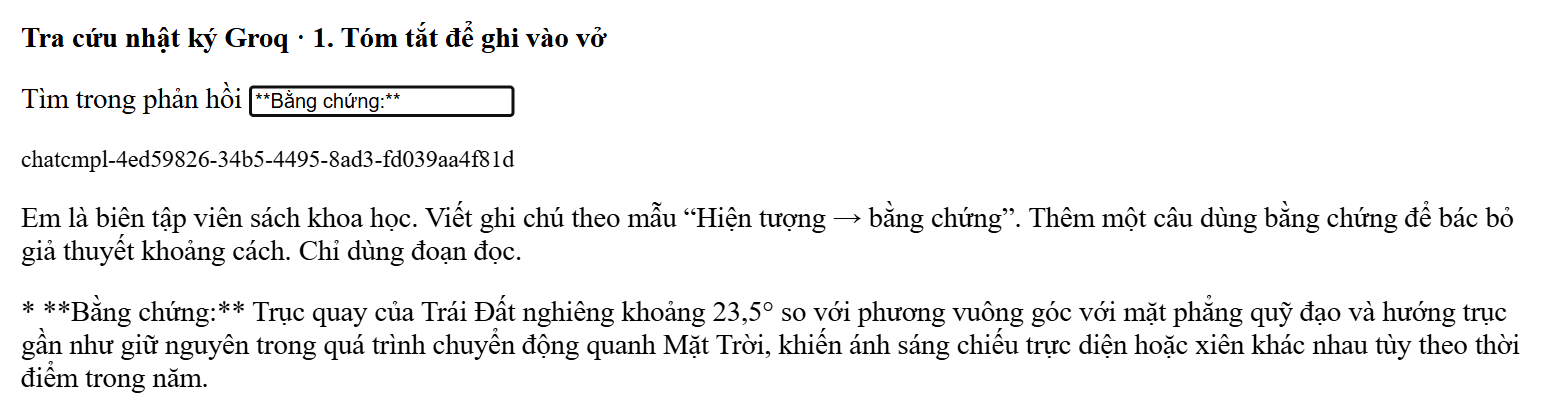
\includegraphics[width=\linewidth]{minh-chung/groq-1.png}\par{\small Hình 1. Trích nhật ký phản hồi nâng cao, kèm mã yêu cầu để đối chiếu với dữ liệu gốc.}
\newpage\section*{2. Giải thích vì sao có mùa}
\small\begin{tabularx}{\linewidth}{@{}p{1.55cm}XX@{}}\hline Mức & Prompt đã gửi & Kết quả quan sát \\ \hline Cơ bản & Vì sao mùa hè thường nóng hơn mùa đông? & Giải thích được hai yếu tố: cùng chùm sáng phủ diện tích nhỏ hơn và ngày dài hơn. Ý về khoảng cách xuất hiện ở cả đầu lẫn cuối. \\[4pt] Cải tiến & Giải thích cho học sinh lớp 6 theo hai ý riêng. Góc chiếu ảnh hưởng thế nào đến cùng một mét vuông đất? Độ dài ngày ảnh hưởng thế nào đến tổng năng lượng nhận được? & Đèn pin giúp hình dung vệt sáng trải rộng. Cụm “thẳng đứng” dễ khiến người đọc tưởng mọi nơi ở Bắc bán cầu đều có Mặt Trời ngay trên đỉnh đầu vào mùa hè. \\[4pt] Nâng cao & Đóng vai giáo viên có một đèn pin và tờ giấy. Hướng dẫn một phép so sánh công bằng để giải thích góc chiếu. Nêu một điều mô hình chưa thể hiện, rồi hỏi một câu để học sinh tự dự đoán. & Giữ khoảng cách đèn–giấy và chỉ ra mô hình chưa thể hiện độ dài ngày. Cuối bài lại quy sự luân phiên ngày đêm cho trục nghiêng. \\[4pt] \hline\end{tabularx}\normalsize\subsection*{Chọn phiên bản nào?}Để trả lời miệng vì sao mùa hè ấm hơn, hai ý trong bản cơ bản đã đủ. Để làm thí nghiệm, bản nâng cao chỉ rõ phải giữ khoảng cách đèn–giấy. Khi giảng lại cần sửa một câu: Trái Đất tự quay tạo nên sự luân phiên ngày đêm; độ nghiêng trục góp phần làm độ dài ngày thay đổi theo mùa. Một thí nghiệm mô tả đúng góc chiếu vẫn có thể đi kèm một lời giải thích sai.\par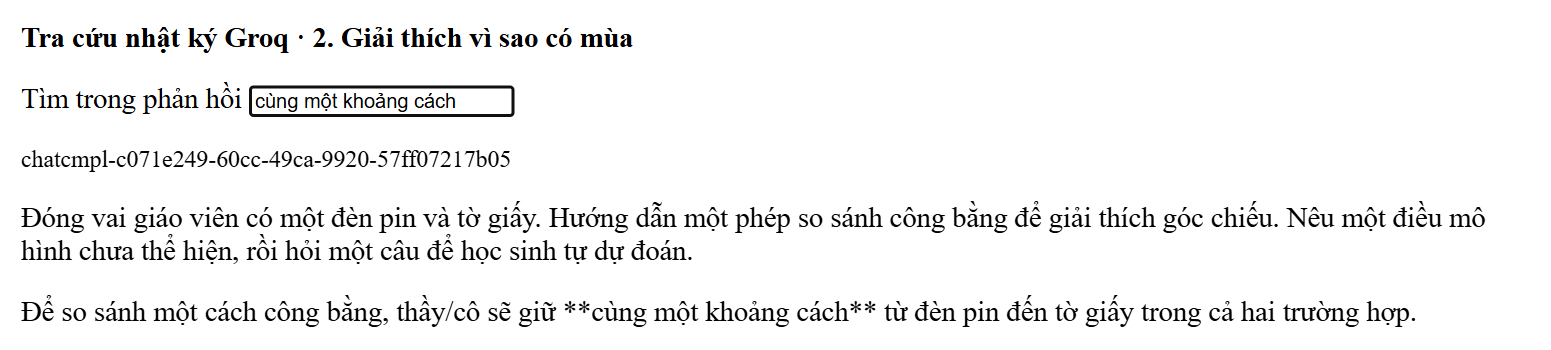
\includegraphics[width=\linewidth]{minh-chung/groq-2.png}\par{\small Hình 2. Trích nhật ký phản hồi nâng cao, kèm mã yêu cầu để đối chiếu với dữ liệu gốc.}
\newpage\section*{3. Tạo câu hỏi tự ôn}
\small\begin{tabularx}{\linewidth}{@{}p{1.55cm}XX@{}}\hline Mức & Prompt đã gửi & Kết quả quan sát \\ \hline Cơ bản & Tạo câu hỏi ôn tập về các mùa. & Tám câu kèm tám đáp án. Đáp án 6 lặp lại kết luận trong ngữ liệu mà chưa giải thích vì sao hai mùa trái ngược là bằng chứng. \\[4pt] Cải tiến & Viết ba câu theo thứ tự nhớ, hiểu, vận dụng. Sau cả ba câu mới ghi đáp án ngắn để em tự chấm. & Có đủ ba câu theo thứ tự yêu cầu, đáp án ở cuối. Câu vận dụng vẫn xoay quanh đúng tình huống tháng Sáu đã học. \\[4pt] Nâng cao & Đóng vai người ra đề. Dùng mẫu “Dự đoán → dẫn chứng” cho một câu vận dụng. Thêm một câu nhớ và một câu chẩn đoán lỗi nhầm về khoảng cách. Gom đáp án cuối bộ, chỉ rõ dấu hiệu trả lời đúng. & Có câu dự đoán cho tháng Mười Hai, câu hỏi độ nghiêng và câu chẩn đoán nhầm lẫn. Đề hỏi thời tiết nhưng đáp án chấm độ dài ngày và góc chiếu. \\[4pt] \hline\end{tabularx}\normalsize\subsection*{Chọn phiên bản nào?}Bản nâng cao thích hợp nhất để tự chấm vì mỗi đáp án nêu dấu hiệu cần có. Nên sửa “hiện tượng thời tiết” thành “độ dài ngày và góc chiếu” cho khớp với đáp án.\par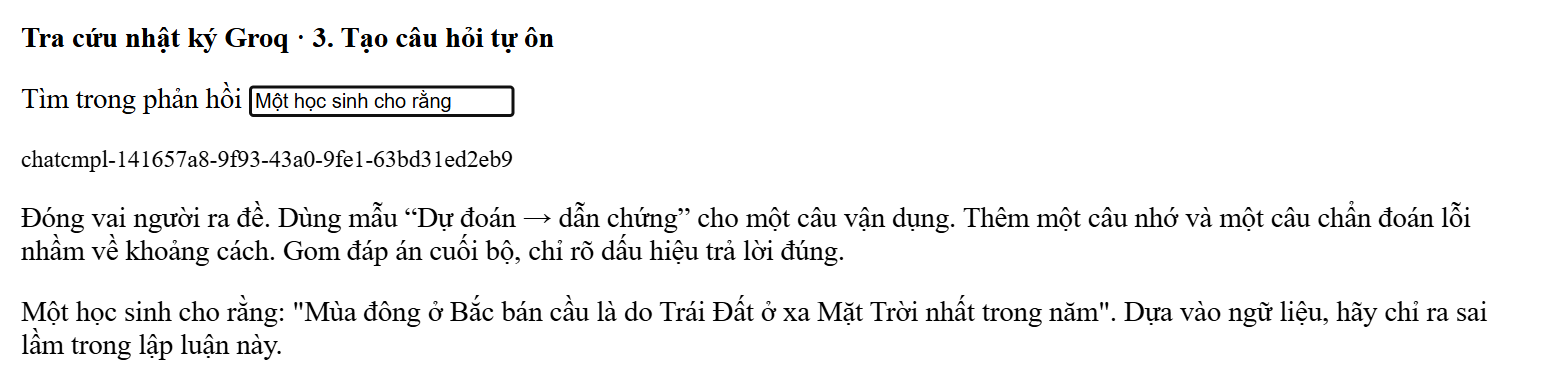
\includegraphics[width=\linewidth]{minh-chung/groq-3.png}\par{\small Hình 3. Trích nhật ký phản hồi nâng cao, kèm mã yêu cầu để đối chiếu với dữ liệu gốc.}
\small\renewcommand{\refname}{Tài liệu tham khảo}\bibliographystyle{unsrt}\bibliography{bibilographic}\end{document}